% ============================================================
% Chapter 20 --- Gram determinants, area and arc length
% Originally: content/week-09.tex, \section{Length, area, and volume} with its
%             subsections (Corsin Week 9). "Volume of embedded surfaces" and "Length of
%             a curve" are promoted to sections here; problems 9.1 and 9.2 join them.
% ============================================================
\chapter{Gram Determinants, Area and Arc Length}
\label{ch:gram_determinant}

% Transition: Claude Opus 5 (Medium)
The previous chapters integrated over subsets of $\mathbb{R}^n$, where the volume element is
just $dx$. This one asks what to integrate over a $d$-dimensional surface sitting inside
$\mathbb{R}^n$, where $d < n$ and there is no such element to start from. The answer runs from
the area of a parallelogram, through the Gram determinant of $m$ vectors in $\mathbb{R}^n$ for
$m \neq n$, to the $d$-volume of a parametrized submanifold --- with the length of a curve as
the case $d = 1$.

% Originally: content/week-09.tex, \section{Length, area, and volume} (Corsin Week 9)

\section{Length, area, and volume}
\label{sec:length_area_volume}

\subsection{The area of a parallelogram in \texorpdfstring{$\mathbb{R}^2$}{R2}}
\label{sec:area_parallelogram}

The relationship between the determinant and volume is a key concept in this part of the
lecture. We illustrate the special case of $\mathbb{R}^2$.

\begin{proposition}[Area of a parallelogram]
\label{prop:area_parallelogram_r2}
Let $x,y \in \mathbb{R}^2$. The area of the parallelogram $(0,x,x+y,y)$ is
\[A = \big|\det(x\mid y)\big|.\]
\end{proposition}

\begin{proof}
Assume w.l.o.g.\ that $x = x_1e_1$, a reduction justified below. Then, writing
$y = (y_1,y_2)\transp$,
\[A = |x_1y_2| = \left|\det\begin{pmatrix} x_1 & y_1 \\ 0 & y_2 \end{pmatrix}\right|,\]
directly from the base-times-height formula for a parallelogram with one side on the
$e_1$-axis.

% Sonnet 5 (Medium) --- FIG-W09-01
\begin{center}
\begin{tikzpicture}[>=Latex, scale=1.0]
  \draw[->] (-0.3,0) -- (3.6,0) node[right, font=\scriptsize] {$e_1$};
  \draw[->] (0,-0.3) -- (0,2.1) node[above, font=\scriptsize] {$e_2$};
  \coordinate (O) at (0,0);
  \coordinate (X) at (2.4,0);
  \coordinate (Y) at (0.7,1.7);
  \coordinate (XY) at (3.1,1.7);
  \draw[purple, dotted, thick] (O) -- (X) -- (XY) -- (Y) -- cycle;
  \draw[blue, thick, ->] (O) -- (X) node[below, font=\scriptsize] {$x=x_1e_1$};
  \draw[orange, thick, ->] (O) -- (Y) node[above left, font=\scriptsize] {$y$};
  \draw[green!50!black, thick, dotted] (Y) -- (0.7,0);
  \draw[green!50!black, ->] (0,-0.15) -- (0.7,-0.15) node[midway, below, font=\scriptsize] {$y_1$};
  \draw[green!50!black, ->] (0.85,0) -- (0.85,1.7) node[midway, right, font=\scriptsize] {$y_2$};
\end{tikzpicture}
\end{center}

For the reduction, let $R \in \operatorname{O}(2)$ be any rotation carrying $x,y$ to a pair
$Rx,Ry$ with $Rx$ along $e_1$; rotations preserve area, so
\[A = \big|\det(Rx\mid Ry)\big| = \big|\det(R)\det(x\mid y)\big| = \big|\det(x\mid y)\big|,\]
using $|\det R| = 1$ and multiplicativity of $\det$. So, the \qt{w.l.o.g.} above was
justified: the formula $A=|\det(x\mid y)|$ holds for the rotated pair, and equals
$|\det(x\mid y)|$ for the original one.
\end{proof}

\subsection{The Gram determinant}
\label{sec:gram_determinant}

\begin{lemma}[Gram determinant of a square matrix]
\label{lem:gram_determinant_square}
For $M \in \mathrm{Mat}_{n\times n}(\mathbb{R})$,
\[|\det(M)| = \sqrt{\det(M)\det(M\transp)} = \sqrt{\det(M\transp)\det(M)}
  = \sqrt{\det(M\transp M)}.\]
\end{lemma}

\begin{proof}
The first equality is $|\det M| = \sqrt{(\det M)^2}$ together with $\det(M\transp)=\det(M)$;
the last is multiplicativity of the determinant, $\det(M\transp)\det(M)=\det(M\transp M)$.
\end{proof}

% Correction: Claude Opus 5 (Ultracode) --- read "the volume ... is given by the Gram
% determinant", which contradicts the ainote immediately below fixing this document's convention:
% the bare $\det(M\transp M)$ is the Gram determinant and its *square root* is the volume. The
% same conflation was repeated at three later sites in this chapter and is corrected there too.
The quantity $\det(M\transp M)$ is called the \newterm{Gram determinant}
\germanfor{Gram-Determinante} of $M$. So, by \cref{prop:area_parallelogram_r2}, the
volume of an $n$-parallelotope in $\mathbb{R}^n$ is given by the \emph{square root} of the Gram
determinant, in analogy to $\lvert\det M\rvert$ itself.

% Supplement: Analysis_II_Script_v1.pdf, p. 119
\begin{ainote}
Terminology diverges from the official script here, worth flagging since it is exactly the kind
of thing that costs a mark in an exam. The script's Definition 13.55 calls $\sqrt{\det(L\transp
L)}$, the square root and so the \emph{volume} itself, the \qt{Gram determinant}. This
document instead follows the more standard usage and calls the bare $\det(M\transp M)$ the Gram
determinant, with the square root then giving the volume (\cref{def:volume_gram_determinant}
below). Every downstream formula agrees regardless of which name is attached to which quantity,
so this is terminology only, not a mathematical disagreement.

The script's own statement of Definition 13.55 is, independently, internally inconsistent: it
introduces a linear map $L:\mathbb{R}^m\to\mathbb{R}^n$ with $m<n$, but then writes the formula
using an undefined $d$ (\qt{the $d\times d$ matrix $L\transp L$}) where the surrounding text
means $m$; and the prose describes \qt{the determinant of the \dots matrix $LL\transp$} while the
displayed formula correctly uses $L\transp L$. Only $L\transp L$ (size $m\times m$) is invertible
for $m<n$, since $LL\transp$ is $n\times n$ and singular. The displayed formula is therefore the
reliable half of the definition, and the surrounding prose is not.
\end{ainote}

\begin{ainote}
The point of restating $|\det M|$ this way is that the middle expression, $\det(M\transp
M)$, still makes sense once $M \in \mathrm{Mat}_{n\times m}(\mathbb{R})$ is rectangular:
$M\transp M \in \mathrm{Mat}_{m\times m}(\mathbb{R})$ is square even when $M$ is not, so its
determinant is always defined, whereas $\det(M)$ itself is not. This is what lets the
notion of \qt{volume spanned by vectors} survive dropping the requirement $m=n$. A set of
fewer than $n$ vectors in $\mathbb{R}^n$ still spans a lower-dimensional parallelotope, and
that parallelotope still has an $m$-dimensional volume, even though no square matrix and no
ordinary determinant is available to compute it with.
\end{ainote}

\begin{definition}[Volume of a parallelotope via the Gram determinant]
\label{def:volume_gram_determinant}
For $m$ vectors $v_1,\dots,v_m \in \mathbb{R}^n$, the \newterm{area}/\newterm{length}/
\newterm{volume} of the parallelotope spanned by them is
\[\sqrt{\det\big(\langle v_i,v_j\rangle\big)} = \sqrt{\det(V\transp V)},
  \qquad V := (v_1\mid v_2\mid\cdots\mid v_m) \in \mathrm{Mat}_{n\times m}(\mathbb{R}).\]
\end{definition}

\begin{example}[$m=1$: the length of a vector]
\label{ex:gram_m1_length}
For $m=1$, $\sqrt{\det(v_1\transp v_1)} = \sqrt{\langle v_1,v_1\rangle} = |v_1|$,
which is the length of $v_1$.
\end{example}

% Source: Corsin Nick/Class Notes/Week 9.pdf, p. 4
\begin{example}[$m=2,\ n=3$: area of a parallelogram in $\mathbb{R}^3$]
\label{ex:gram_m2_n3_area}
For $m=2$, $n=3$, we hope that the Gram determinant of
\[M = \begin{pmatrix} x_1 & y_1 \\ x_2 & y_2 \\ x_3 & y_3 \end{pmatrix}\]
gives the area of the parallelogram spanned by $x$ and $y$ in $\mathbb{R}^3$. If $\theta$ is
the angle between $x$ and $y$, this should be $A = |x|\,|y|\,|\sin\theta|$.

% Sonnet 5 (Medium) --- FIG-W09-02
% Correction: Gemini 3.7 Flash (High) --- dropped altitude was vertical rather than perpendicular
% to y (angle 81.6 deg); now drops perpendicularly to proj_y(x) = (2.79, 0.41) on the dashed line of y.
% Correction: Claude Opus 5 (Ultracode), found by rendering printed p. 314 --- that fix was right
% and incomplete. Three things follow it.
%   * The $|x|\sin\theta$ label had no plate, and the purple edge $XY \to Y$ runs straight through
%     it: that edge is $y = 0.25 + 0.6538(x-1.7)$, which crosses the label's own height $y = 1.05$
%     at $x = 2.92$, inside the label's span. Printed, the bar and the $x$ of $|x|$ came out
%     struck through. It takes the `lbl' plate from style.md. (The strikethrough predates the
%     altitude fix -- at the old position $(2.68,1.0)$ the same edge crossed at $x = 2.847$ --
%     but the label was moved without checking the page.)
%   * The $\theta$ arc annotates the very angle the altitude depends on and was left unaudited.
%     `(0.55,0.075) arc (5:33:0.6)' starts at radius $0.5551$, so TikZ centres the arc at
%     $(0.55,0.075) - 0.6(\cos 5^\circ, \sin 5^\circ) = (-0.048, 0.023)$, not at the origin; and
%     it spans $5^\circ$ to $33^\circ$ where the true directions are
%     $\arctan(0.25/1.7) = 8.37^\circ$ and $\arctan(1.7/2.6) = 33.17^\circ$. Restarted from
%     $0.6(\cos 8.37^\circ, \sin 8.37^\circ) = (0.5936, 0.0873)$, which puts the centre on $O$ and
%     the ends on $y$ and $x$. This is the idiom `02-metric-normed-inner-product/03-cauchy-schwarz'
%     already uses correctly (`arc (14:59:0.5)' against $14.04^\circ$ and $59.04^\circ$).
%   * A right-angle mark at the foot, so the perpendicularity the fix installed is visible rather
%     than merely true. Unit vector along $y$ is $(0.9893, 0.1455)$; the mark is drawn at side
%     $0.12$ from the foot back along $-y$ and up along the perpendicular $(-0.1455, 0.9893)$.
\begin{center}
\begin{tikzpicture}[>=Latex, scale=1.3,
  lbl/.style={fill=white, fill opacity=0.85, text opacity=1, inner sep=1.2pt,
              rounded corners=1pt}]
  \coordinate (O) at (0,0);
  \coordinate (X) at (2.6,1.7);
  \coordinate (Y) at (1.7,0.25);
  \coordinate (XY) at (4.3,1.95);
  \draw[orange, thick, ->] (O) -- (Y) node[below right, font=\scriptsize] {$y$};
  \draw[gray!55, dashed] (Y) -- (3.05,0.45);
  \draw[blue, thick, ->] (O) -- (X) node[above, font=\scriptsize] {$x$};
  \draw[purple, dotted, thick] (X) -- (XY) -- (Y);
  % Dashed, not dotted: the parallelogram's own edges above are thick dotted, and red against
  % purple is a distinction in hue alone, which style.md forbids relying on -- an e-reader renders
  % both as the same grey. The dash pattern, the right-angle mark and the label are the three
  % channels that now separate the altitude from the edge it runs beside.
  \draw[red, dashed, thick] (X) -- (2.79,0.41);
  \draw[red] (2.6713,0.3925) -- (2.6538,0.5112) -- (2.7725,0.5287);
  \node[lbl, text=red, font=\scriptsize, right] at (2.75,1.05) {$|x|\sin\theta$};
  \draw (0.5936,0.0873) arc (8.37:33.17:0.6);
  \node[font=\scriptsize] at (0.9,0.32) {$\theta$};
\end{tikzpicture}
\end{center}

And indeed:
\[
\begin{aligned}
\sqrt{\det(M\transp M)}
  &= \sqrt{\det\begin{pmatrix} \langle x,x\rangle & \langle x,y\rangle \\
    \langle x,y\rangle & \langle y,y\rangle\end{pmatrix}} \\
  &= \sqrt{\langle x,x\rangle\langle y,y\rangle - \langle x,y\rangle^2} \\
  &= \sqrt{|x|^2|y|^2 - |x|^2|y|^2\cos^2\theta} \\
  &= |x|\,|y|\,|\sin\theta| \qquad (=\ |x\times y|).
\end{aligned}
\]
\end{example}

% Originally: content/week-09.tex, \subsection{Volume of embedded surfaces} --- promoted to a section

\section{Volume of embedded surfaces}
\label{sec:volume_embedded_surfaces}

% Source: Corsin Nick/Class Notes/Week 9.pdf, p. 5
% Def. 13.68
\begin{definition}[$d$-volume on a parametrized $d$-submanifold]
\label{def:d_volume_parametrized_submanifold}
Let $V \subseteq \mathbb{R}^d$ be open, and let $\phi : V \to \mathbb{R}^n$ be a parametrized
submanifold. Given a Jordan measurable set $E \subseteq V$ with $\overline E \subseteq V$,
we define the $d$-volume of $\phi(E)$ by
\[\vol_d(\phi(E)) := \int_E \sqrt{\det\big(D\phi(x)\transp D\phi(x)\big)}\,dx.\]
\end{definition}

Here the Gram determinant in the integrand is the volume of the parallelotope spanned by the
vectors $\partial_1\phi(x),\partial_2\phi(x),\dots,\partial_d\phi(x)$, which by assumption
(see \qt{parametrized submanifold}) are linearly independent, i.e.\ $D\phi(x)$ has full rank,
so the volume is strictly positive.

% Sonnet 5 (Medium) --- FIG-W09-03
\begin{center}
\begin{tikzpicture}[>=Latex, scale=1.3]
  \draw[thick] plot[smooth] coordinates {(-2.1,-0.4) (-0.8,0.65) (0.5,-0.15) (2.1,0.75)};
  \draw[thick] plot[smooth] coordinates {(-1.8,0.9) (-0.5,-0.5) (0.8,0.4) (2.3,-0.65)};
  \coordinate (P) at (0.0,0.05);
  \fill (P) circle (1.6pt) node[below left, font=\scriptsize] {$\phi(x)$};
  \draw[blue, thick, ->] (P) -- ++(1.2,0.4) coordinate (D1)
    node[right, font=\scriptsize] {$\partial_1\phi(x)$};
  \draw[purple, thick, ->] (P) -- ++(0.35,1.05) coordinate (D2)
    node[above, font=\scriptsize] {$\partial_2\phi(x)$};
  \draw[green!55!black, dashed]
    (D1) -- ++(0.35,1.05) -- (D2) -- cycle;
  \node[green!45!black, font=\scriptsize, align=center] at (2.1,1.5)
    {$\sqrt{\det(D\phi(x)\transp D\phi(x))}$};
  \draw[green!55!black, thin, ->] (1.55,1.3) -- (0.95,1.0);
\end{tikzpicture}
\end{center}

This factor gives a measure for the stretching of $E$ as it is \qt{glued} to the surface. If
\[\sqrt{\det\big(D\phi(x)\transp D\phi(x)\big)} = 1 \quad \text{for all } x,\]
then $\phi$ is called an \newterm{isometry} (\germanterm{Isometrie}). A special case is the
length of a curve, treated in \cref{sec:length_of_curve} below.

% Quelle: Linus Lüchinger/Slides/Slides-04-20.pdf, slide 14
% Generator: Claude Opus 5 (High)
\begin{remark}[Why the transpose, and why the square root]
\label{rem:why_gram_determinant}
The shape of the formula looks arbitrary until one asks what could possibly stand in its place.
The honest question is: \emph{by what factor does $\phi$ stretch $d$-dimensional volume near
$x$?} Near $x$ the map $\phi$ is its differential, so the question is really about the linear
map $D\phi(x)$, and the answer runs in three steps.
\begin{enumerate}[label=\textbf{(\alph*)}]
  \item \textbf{The obvious candidate does not exist.} For a map $\mathbb{R}^n \to \mathbb{R}^n$
    the stretching factor is $\lvert\det\rvert$. Here $D\phi(x)$ is $n \times d$ with $d < n$, a
    \emph{rectangular} matrix, and a rectangular matrix has no determinant. So, the one-line
    answer is unavailable, and something has to replace it.
  \item \textbf{A factor nevertheless exists.} A linear map still scales all $d$-volumes in its
    domain by one and the same constant: it sends the unit cube of $\mathbb{R}^d$ to a fixed
    parallelotope, and every other region is built from scaled copies of that cube. Call this
    constant $c \geq 0$. It is what we want; we only need a formula for it.
  \item \textbf{The Gram matrix supplies it.} The product $D\phi(x)\transp D\phi(x)$ is
    $d \times d$, square at last, so it \emph{does} have a determinant, and that
    determinant turns out to be exactly $c^2$. Hence $c = \sqrt{\det(D\phi\transp D\phi)}$, and
    the square root is there for no deeper reason than to undo that squaring.
\end{enumerate}
The two familiar formulas are the small cases. For $d=1$ the matrix $D\phi(t)$ is the single
column $\phi'(t)$, so $D\phi\transp D\phi = \lvert\phi'(t)\rvert^2$ and $c = \lvert\phi'(t)\rvert$,
which is the arc-length integrand of \cref{sec:length_of_curve}. For $d=2$, $n=3$ one computes
$c = \lvert\partial_1\phi \times \partial_2\phi\rvert$, the area of the parallelogram the two
tangent vectors span, which is the surface-area formula used throughout this chapter.
\end{remark}

% Quelle: Linus Lüchinger/Slides/Slides-04-20.pdf, slide 12
\begin{ainote}[Two objects, three notations]
From this chapter onwards the lecture notes write $D\phi(x)$ for the Jacobian \emph{matrix} of
$\phi$ at $x$, the object earlier chapters of this document call $\Jac\phi(x)$. That collides
with the notation $D\phi_x$ used since \cref{ch:differential} for the \emph{differential}, the
linear map itself. The two are not the same kind of object, even though they carry the same
information:
\[\underbrace{D\phi_x}_{\text{linear map}}(v) \;=\; \underbrace{\Jac\phi(x)}_{\text{matrix}}\,v
  \;=\; \underbrace{D\phi(x)}_{\text{same matrix}}\,v.\]
The subscript is the whole distinction: $D\phi_x$ has $x$ downstairs, $D\phi(x)$ has it in
brackets. This document keeps each source's own convention rather than renotating transcribed
material, so both spellings of the matrix appear; where it matters, read $D\phi(x)$ and
$\Jac\phi(x)$ as synonyms.
\end{ainote}

% Supplement: Sascha Brack/Class Notes/Week_09_Notes_Friday.pdf, p. 3
\begin{example}[Integral on the graph of a function]
\label{ex:integral_graph_function}
Given an open set $U \subseteq \mathbb{R}^2$ and a $C^1$ function $f: U \to \mathbb{R}$, we can define the parametrized surface $\phi: U \to \mathbb{R}^3$ by $\phi(x,y) = (x,y,f(x,y))\transp$.
Assuming $M := \operatorname{Im}\phi$ is a $C^1$ submanifold, its area is given by $\int_M 1 \mathop{d\text{vol}}_2$.

We first find the Jacobian matrix of the parametrization:
\[\Jac\phi(x,y) = \begin{pmatrix} 1 & 0 \\ 0 & 1 \\ \partial_1 f(x,y) & \partial_2 f(x,y) \end{pmatrix}.\]
Then we compute the Gram determinant:
\begin{align*}
\sqrt{|\det(\Jac\phi\transp \Jac\phi)|}
&= \sqrt{\det \begin{pmatrix} 1+(\partial_1 f)^2 & \partial_1 f \partial_2 f \\ \partial_2 f \partial_1 f & 1+(\partial_2 f)^2 \end{pmatrix}} \\
&= \sqrt{\big(1+(\partial_1 f)^2\big)\big(1+(\partial_2 f)^2\big) - (\partial_1 f)^2(\partial_2 f)^2} \\
&= \sqrt{1 + (\partial_1 f)^2 + (\partial_2 f)^2} = \sqrt{1+|\nabla f(x,y)|^2}.
\end{align*}
By definition, we get the surface area formula for a graph:
\[\int_M 1 \mathop{d\text{vol}}_2 = \int_U \sqrt{1+|\nabla f(x,y)|^2} \,dx\,dy.\]
\end{example}

\subsection{Example: area of a paraboloid patch}
\label{sec:example_paraboloid_area}

% Source: Corsin Nick/Class Notes/Week 9.pdf, pp. 6--7
\begin{example}[Area of a paraboloid patch]
\label{ex:paraboloid_patch_area}
Compute the area of the surface
\[F = \left\{(x,y,z)\in\mathbb{R}^3 \ :\ x^2+4y^2 < 8,\ \ z = \tfrac12(x^2+2y^2)\right\}.\]

Since $z = \tfrac12(x^2+2y^2)$ means $F$ is a graph, we can conveniently write $F$ as the
image of the parametrization
\[\phi : A \to F, \qquad (x,y) \mapsto \left(x,\,y,\,\tfrac12(x^2+2y^2)\right),
  \qquad A := \{(x,y)\in\mathbb{R}^2 : x^2+4y^2 < 8\}.\]

\textbf{Gram determinant.} We compute
\[D\phi(x,y) = \begin{pmatrix} 1 & 0 \\ 0 & 1 \\ x & 2y \end{pmatrix}
  \quad \Longrightarrow \quad
  D\phi(x,y)\transp D\phi(x,y) = \begin{pmatrix} 1+x^2 & 2xy \\ 2xy & 1+4y^2 \end{pmatrix},\]
so that
\[\sqrt{\det D\phi(x,y)\transp D\phi(x,y)}
  = \sqrt{(1+x^2)(1+4y^2) - 4x^2y^2}
  = \sqrt{1+x^2+4y^2}.\]

\textbf{The integral.} By \cref{def:d_volume_parametrized_submanifold},
\[\vol_2(F) = \int_A \sqrt{1+x^2+4y^2}\,dx\,dy, \qquad A = \{(x,y)\in\mathbb{R}^2 :
x^2+4y^2<8\}.\]

We should choose more convenient coordinates. Polar coordinates come to mind, but then we
still have problems, since $A$ is not radially symmetric. We want to write
$A = \Psi\big((0,R)\times(0,2\pi)\big)$ (up to a set of measure zero). Note that for $y=0$,
$|x| < \sqrt8 = 2\sqrt2$, and for $x=0$, $|y| < \sqrt2$. Choosing $R := \sqrt2$ and weighing
$x,y$ accordingly,
\[\begin{pmatrix} x \\ y \end{pmatrix} = \begin{pmatrix} 2r\cos\theta \\ r\sin\theta
\end{pmatrix} =: \Psi(r,\theta).\]

\textbf{Change of variables.}
\[dx\,dy = |\det D\Psi(r,\theta)|\,dr\,d\theta
  = \left\lVert \begin{matrix} 2\cos\theta & -2r\sin\theta \\ \sin\theta & r\cos\theta
    \end{matrix}\right\rVert dr\,d\theta = 2r\,dr\,d\theta,\]
giving
\[
\begin{aligned}
\vol_2(F) &= \int_A \sqrt{1+x^2+4y^2}\,dx\,dy
  = \int_0^{\sqrt2} dr\int_0^{2\pi} d\theta\ 2r\sqrt{1+4r^2} \\
  &= 4\pi\int_0^{\sqrt2} dr\ r(1+4r^2)^{1/2}
   = \frac\pi2\int_0^{\sqrt2} dr\ 8r(1+4r^2)^{1/2} \\
  &= \frac\pi2\left[(1+4r^2)^{3/2}\cdot\frac23\right]_0^{\sqrt2}
   = \frac\pi3\big(27-1\big) = \frac{26\pi}{3}.
\end{aligned}
\]
\end{example}

\begin{ainote}
Worth flagging what makes $A$ awkward: it is an ellipse, not a disc, so naive polar
coordinates $(x,y)=(\rho\cos\theta,\rho\sin\theta)$ would force $\rho$ to depend on $\theta$
along the boundary. The fix is to build the eccentricity into the change of variables itself.
Scaling $x$ by a factor of $2$ relative to $y$ turns the ellipse into the disc $r<\sqrt2$
before polar coordinates are even applied. This is the same idea as
\Cref{ex:change_of_variables_domain}: choose $\Psi$ to straighten the domain, not
to simplify the integrand.
\end{ainote}

% Supplement: Sascha Brack/Class Notes/Week_09_Notes_Monday.pdf, p. 7
\begin{example}[Surface area of a sphere]
\label{ex:surface_area_sphere}
Given the sphere $M := \{(x,y,z) \in \mathbb{R}^3 \mid x^2+y^2+z^2 = r^2\}$, we can use the parametrization $\phi : (0,\pi) \times (-\pi,\pi) \to \mathbb{R}^3$,
\[\phi(\theta,\varphi) = \begin{pmatrix} r\sin\theta\cos\varphi \\ r\sin\theta\sin\varphi \\ r\cos\theta \end{pmatrix}.\]
The Jacobian matrix is
\[\Jac\phi(\theta,\varphi) = \begin{pmatrix} r\cos\theta\cos\varphi & -r\sin\theta\sin\varphi \\ r\cos\theta\sin\varphi & r\sin\theta\cos\varphi \\ -r\sin\theta & 0 \end{pmatrix},\]
which has rank 2 for all $(\theta,\varphi)$ in the domain.
Then we compute the Gram determinant:
\[\Jac\phi\transp \Jac\phi = \begin{pmatrix} r^2 & 0 \\ 0 & r^2\sin^2\theta \end{pmatrix} \quad \Longrightarrow \quad \sqrt{\det(\Jac\phi\transp \Jac\phi)} = r^2\sin\theta.\]
The surface area is given by the integral:
\begin{align*}
\int_M 1 \mathop{d\text{vol}}_2 &= \int_{-\pi}^\pi \int_0^\pi \sqrt{\det(\Jac\phi\transp \Jac\phi)} \,d\theta\,d\varphi \\
&= \int_{-\pi}^\pi \int_0^\pi r^2\sin\theta \,d\theta\,d\varphi \\
&= r^2 \left(\int_{-\pi}^\pi d\varphi\right) \left(\int_0^\pi \sin\theta \,d\theta\right) \\
&= r^2 \cdot 2\pi \cdot 2 = 4\pi r^2.
\end{align*}
Note that here, our partition of unity simply was the identity (since the parametrization covers the sphere up to a null set).

\begin{center}
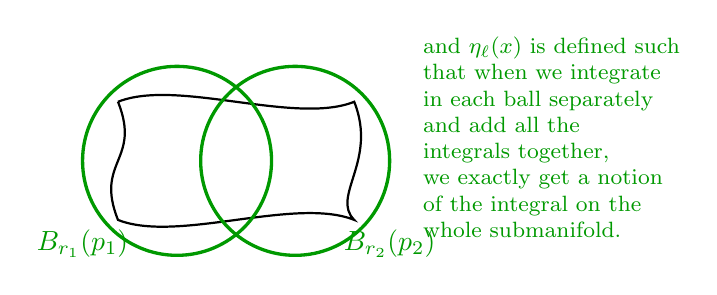
\begin{tikzpicture}[scale=1.5]
  % Submanifold shape
  \draw[thick] (0,0) .. controls (0.5,0.2) and (1.5,-0.2) .. (2,0)
               .. controls (2.2,-0.5) and (1.8,-0.8) .. (2,-1)
               .. controls (1.5,-0.8) and (0.5,-1.2) .. (0,-1)
               .. controls (-0.2,-0.5) and (0.2,-0.5) .. (0,0);
               
  % Two charts
  \draw[very thick, green!60!black] (0.5,-0.5) circle (0.8);
  \node[green!60!black] at (-0.3,-1.2) {$B_{r_1}(p_1)$};
  
  \draw[very thick, green!60!black] (1.5,-0.5) circle (0.8);
  \node[green!60!black] at (2.3,-1.2) {$B_{r_2}(p_2)$};
  
  \node[right, font=\footnotesize, align=left, text=green!60!black] at (2.5, -0.3) {
    and $\eta_\ell(x)$ is defined such\\
    that when we integrate\\
    in each ball separately\\
    and add all the\\
    integrals together,\\
    we exactly get a notion\\
    of the integral on the\\
    whole submanifold.
  };
\end{tikzpicture}
\end{center}
\end{example}


% --- exercises relocated here from the dissolved sheet 9 ---

% Originally: content/week-09.tex, \exercisesheet{9}, problem 9.1
% Source: exercises/Ex9_Analysis2_eng.pdf

% Source: exercises/Ex9_Analysis2_eng.pdf, p. 1
\begin{exercise}[9.1 --- Volume \textnormal{(important)}]
\label{ex:9.1}
Calculate the volume of the region $B \subset \mathbb{R}^3$ enclosed by the surfaces
$x^2+y^2+z^2=8$ and $2z=x^2+y^2$. \textit{Official hint:} use cylindrical coordinates.

% Source: Corsin Nick/Class Notes/Week 9.pdf, p. 1
\textit{Corsin's hint:}
\[\begin{pmatrix} x \\ y \\ z\end{pmatrix} = \begin{pmatrix} r\sin\theta\cos\varphi \\
  r\sin\theta\sin\varphi \\ r\cos\theta \end{pmatrix}
  \qquad \text{for } (r,\theta,\varphi) \in (0,\infty)\times(0,\pi)\times(0,2\pi).\]
\end{exercise}

% The solution in 99-solutions.tex points back at this note, so it carries a label. Possible
% only since 2026-08-09, when ainote gained its own counter; the solution used to say
% "see the \texttt{ainote} above", which leaked a LaTeX environment name into the typeset text.
\begin{ainote}[Corsin's hint is spherical, not cylindrical]
\label{note:9.1_coordinates_mislabelled}
Corsin labels the formula above \qt{cylindrical coordinates}, but $(r\sin\theta\cos\varphi$, $r\sin\theta\sin\varphi$, $r\cos\theta)$ is the \textbf{spherical} parametrization, and his
range $\theta \in (-\pi/2,\pi/2)$ has been corrected to $(0,\pi)$, the range on which
$\theta \mapsto \cos\theta$ actually covers $[-1,1]$ bijectively (already logged in \cref{ex:7.6}). The mislabelling is doubly worth noting here, since the official sheet's own hint
recommends \emph{cylindrical} coordinates $(r,\theta,z)$, and that is in fact the more
natural choice for this problem, as the solution on \cpageref{ex:solution_9.1} does: both surfaces are
surfaces of revolution about the $z$-axis, which cylindrical coordinates respect directly,
whereas spherical coordinates mix $r$ and $\theta$ into both defining equations.
\end{ainote}

% Originally: content/week-10.tex, \exercisesheet{10}, problem 10.1
% Source: exercises/Ex10_Analysis2_eng.pdf

% Source: exercises/Ex10_Analysis2_eng.pdf, p. 1
\begin{exercise}[10.1 --- Spherical quadrilateral \textnormal{(important)}]
\label{ex:10.1}
Calculate the area of the spherical quadrilateral $S \subset \mathbb{S}^2$ bounded by the
meridians $-\pi < \varphi_1 < \varphi_2 < \pi$ and parallels $-\pi/2 < \theta_1 < \theta_2 <
\pi/2$.
\end{exercise}

% Originally: content/week-10.tex, \exercisesheet{10}, problem 10.2
% Source: exercises/Ex10_Analysis2_eng.pdf

% Source: exercises/Ex10_Analysis2_eng.pdf, p. 1
\begin{exercise}[10.2 --- The surface area of a torus \textnormal{(important)}]
\label{ex:10.2}
Let $S := \{(x,y,0)\in\mathbb{R}^3 \mid x^2+y^2=4\}$ and $T := \{x\in\mathbb{R}^3 \mid d_S(x)
\leq 1\}$, where $d_S(x) = \inf\{\lvert x-y\rvert \mid y\in S\}$ denotes the minimal distance
from $S$ to $x\in\mathbb{R}^3$. Parametrize $\partial T$ and then calculate the area.

% Source: Corsin Nick/Class Notes/Week 10.pdf, p. 1
\textit{Corsin's hint, general parametrization of a torus surface:}
\[x = (R+r\cos\phi)\cos\theta, \qquad y = (R+r\cos\phi)\sin\theta, \qquad z = r\sin\phi,\]
for the torus swept by a tube of radius $r$ at distance $R$ from the axis.

% Sonnet 5 (Medium) --- FIG-W10-01
\begin{center}
\begin{tikzpicture}[>=Latex, scale=1.0]
  \begin{scope}
    \draw[->] (0,0) -- (2.2,0) node[right, font=\scriptsize] {$x$};
    \draw[->] (0,0) -- (0,1.8) node[above, font=\scriptsize] {$z$};
    \draw[->] (0,0) -- (-1.1,-0.7) node[left, font=\scriptsize] {$y$};
    \draw[blue!70!black, thick] (0.4,0.55) circle (0.9 and 0.35);
    \draw[blue!70!black, thick] (0.05,0.15) circle (1.5 and 0.6);
    \draw[blue!70!black, dashed] (-1.0,0.0) arc (180:360:1.5 and 0.6);
  \end{scope}
  \begin{scope}[xshift=5.2cm]
    \draw[blue!70!black, thick] (0,0) circle (1.6);
    \draw[blue!70!black, thick] (0,0) circle (0.7);
    \draw[->] (0,0) -- (55:1.15) node[midway, above, font=\scriptsize] {$R$};
    \draw[orange, ->] (0,0) -- (18:0.7) node[midway, below, font=\scriptsize] {};
    \draw[orange, thick, ->] (18:0.7) -- (55:1.6)
      node[midway, above right, font=\scriptsize] {$r$};
    \draw (0.55,0) arc (0:18:0.55);
    \node[font=\scriptsize] at (0.75,0.15) {$\theta$};
    \draw[->] (1.1,0) -- (2.0,0) node[right, font=\scriptsize] {$x$};
    \draw[->] (1.1,0) -- (1.1,0.9) node[above, font=\scriptsize] {$y$};
  \end{scope}
  \begin{scope}[xshift=10.4cm]
    \draw[purple, dotted] (-1.6,0) -- (1.6,0);
    \draw (0,0) circle (0.9);
    \draw[->] (0,0) -- (35:0.9) node[midway, above right, font=\scriptsize] {$r$};
    \draw (0.35,0) arc (0:35:0.35);
    \node[font=\scriptsize] at (0.55,0.15) {$\varphi$};
    \draw[->] (-1.6,-0.3) -- (-1.6,0.9) node[above, font=\scriptsize] {$z$};
    \draw[->] (-1.6,-0.3) -- (-0.6,-0.3) node[right, font=\scriptsize] {$x$};
  \end{scope}
\end{tikzpicture}
\end{center}
\end{exercise}

% Originally: content/week-09.tex, \subsection{Length of a curve} --- promoted to a section

\section{Length of a curve}
\label{sec:length_of_curve}

% Source: Corsin Nick/Class Notes/Week 9.pdf, p. 8
\begin{definition}[Length of a $C^1$-curve]
\label{def:length_c1_curve}
The \newterm{length} \germanfor{Länge} of a curve or path $\gamma \in
C^1([a,b],\mathbb{R}^n)$ is given by
\[L(\gamma) := \int_a^b \lvert\gamma'(t)\rvert\,dt.\]
\end{definition}

\begin{definition}[Length of a $C^0$-curve]
\label{def:length_c0_curve}
For a $C^0$-curve $c \in C^0([a,b],\mathbb{R}^n)$, the length is defined as
\[L(c) := \sup\left\{\sum_{i=1}^{n-1} \lvert c(t_{i+1})-c(t_i)\rvert
  \ :\ a = t_1 < \cdots < t_n = b\right\},\]
the supremum over all lengths of inscribed polygons.
\end{definition}

% Sonnet 5 (Medium) --- FIG-W09-04
\begin{center}
\begin{tikzpicture}[>=Latex, scale=1.0]
  \draw[thick] plot[smooth] coordinates
    {(0,0) (0.6,0.9) (1.3,0.5) (1.9,0.15) (2.5,0.75) (3.1,0.5) (3.7,1.3)};
  \node[font=\scriptsize] at (1.9,1.15) {$\operatorname{Im}(c)$};
  \draw[blue, thick]
    (0,0) -- (0.55,0.95) -- (1.35,0.55) -- (2.0,0.1) -- (2.55,0.7) -- (3.15,0.45) -- (3.7,1.25);
  \foreach \x/\y/\lbl/\pos in {0/0/{c(t_1)}/below,0.55/0.95/{c(t_2)}/above,1.35/0.55/{c(t_3)}/above,2.0/0.1/{c(t_4)}/below,2.55/0.7/{c(t_5)}/{above left},3.15/0.45/{c(t_6)}/below,3.7/1.25/{c(t_7)}/right} {
    \fill (\x,\y) circle (1.3pt);
    \node[font=\scriptsize, \pos] at (\x,\y) {$\lbl$};
  }
\end{tikzpicture}
\end{center}

\begin{remark}
For a $C^1$-curve, \cref{def:length_c1_curve,def:length_c0_curve} agree. Notice that
\[\lvert\gamma'(t)\rvert = \sqrt{D\gamma(t)\transp \cdot D\gamma(t)}\]
is exactly the Gram determinant of $D\gamma(t)$ in the sense of
\Cref{def:volume_gram_determinant}, the $m=1$ case of \cref{ex:gram_m1_length}, now applied
pointwise along the curve. This is why the length of a curve is the special case
$d=1$ of \cref{def:d_volume_parametrized_submanifold}: a curve is a $1$-dimensional
parametrized submanifold, and $L(\gamma) = \vol_1(\gamma([a,b]))$.
\end{remark}

% Supplement: Sascha Brack/Class Notes/Week_09_Notes_Friday.pdf, p. 4
\begin{example}[Line integral]
\label{ex:line_integral}
Let $\phi : [-\pi/2, \pi/2] \to \mathbb{R}^2$ be given by $\phi(\theta) = \begin{pmatrix} 3\sin\theta \\ 4\sin\theta \end{pmatrix}$.
Compute the length of the curve $M := \operatorname{Im}\phi$, i.e.\ $\int_M 1 \mathop{d\text{vol}}_1$.

First, we compute the Jacobian (which here is just the derivative vector):
\[\Jac\phi(\theta) = \begin{pmatrix} 3\cos\theta \\ 4\cos\theta \end{pmatrix}.\]
Then we compute the Gram determinant (which is the length of the tangent vector):
\[\sqrt{\det(\Jac\phi(\theta)\transp \Jac\phi(\theta))} = \sqrt{9\cos^2\theta + 16\cos^2\theta} = \sqrt{25\cos^2\theta} = 5|\cos\theta|.\]
Since $\cos\theta \geq 0$ for $\theta \in [-\pi/2, \pi/2]$, this simplifies to $5\cos\theta$.
The length is:
\[\int_{-\pi/2}^{\pi/2} 5\cos\theta \,d\theta = 5\big[\sin\theta\big]_{-\pi/2}^{\pi/2} = 5(1 - (-1)) = 10.\]
\end{example}

% Source: Linus Lüchinger/Slides/Slides-04-30.pdf, p. 4
\begin{proposition}[Length of a graph]
\label{prop:graph_arc_length}
Let $f \in C^1([a,b],\mathbb{R})$. The graph
$\Gamma_f := \{(x,f(x)) : x \in [a,b]\} \subseteq \mathbb{R}^2$ has length
\[\vol_1(\Gamma_f) = \int_a^b \sqrt{1+f'(x)^2}\,dx.\]
\end{proposition}

\begin{proof}
Parametrize by $\phi(t) := (t, f(t))\transp$ on $[a,b]$, which is injective and $C^1$ with
$\phi'(t) = (1, f'(t))\transp \neq 0$. The Gram determinant of the single tangent vector is
\[\sqrt{\det\big(\Jac\phi(t)\transp\Jac\phi(t)\big)} = |\phi'(t)|
  = \sqrt{1+f'(t)^2},\]
and integrating over $[a,b]$ is the definition of $\vol_1$.
\end{proof}

% Source: Linus Lüchinger/Slides/Slides-04-30.pdf, p. 4
\begin{example}[A quarter of an astroid]
\label{ex:astroid_arc_length}
Let $\gamma(t) := (\cos^3t,\ \sin^3t)\transp$ for $t \in [0,\tfrac\pi2]$. Then
\[\gamma'(t) = \begin{pmatrix} -3\cos^2t\,\sin t \\ 3\sin^2t\,\cos t\end{pmatrix},\]
so, using $\cos t \geq 0$ and $\sin t \geq 0$ on this interval,
\[|\gamma'(t)| = 3\cos t\,\sin t\sqrt{\cos^2t+\sin^2t} = 3\cos t\,\sin t
  = \tfrac32\sin(2t).\]
The length is therefore
\[\int_0^{\pi/2}\tfrac32\sin(2t)\,dt = \Big[-\tfrac34\cos(2t)\Big]_0^{\pi/2}
  = -\tfrac34\big((-1)-1\big) = \tfrac32.\]
Note that $\gamma'(0) = \gamma'(\tfrac\pi2) = 0$: the astroid has cusps at its endpoints, so this
is a curve whose parametrization fails the immersion condition exactly at the two boundary
points. The length integral is unaffected, since two points contribute nothing to it.
\end{example}

% Supplement: Sascha Brack/Class Notes/Week_09_Notes_Friday.pdf, p. 6
\begin{example}[Spiral length]
\label{ex:spiral_length}
Consider the spiral parametrized by $\phi : (0,2\pi) \to \mathbb{R}^3$,
\[\phi(t) = \begin{pmatrix} \cos(\omega t) \\ \sin(\omega t) \\ vt \end{pmatrix},\]
where $v \in \mathbb{R}\setminus\{0\}$ and $\omega \in (0,\infty)$. Compute the length of the spiral $\operatorname{Im}\phi$.

We compute the Jacobian:
\[\Jac\phi(t) = \begin{pmatrix} -\omega\sin(\omega t) \\ \omega\cos(\omega t) \\ v \end{pmatrix}.\]
The Gram determinant is:
\[\sqrt{\Jac\phi(t)\transp \Jac\phi(t)} = \sqrt{\omega^2\sin^2(\omega t) + \omega^2\cos^2(\omega t) + v^2} = \sqrt{\omega^2 + v^2}.\]
The length of the spiral is the integral over the parameter domain:
\[\int_0^{2\pi} \sqrt{\omega^2 + v^2} \,dt = 2\pi\sqrt{\omega^2 + v^2}.\]
\end{example}

% Supplement: Sascha Brack/Class Notes/Week_09_Notes_Monday.pdf, p. 8
\begin{example}[Line integral of a function on a circle]
\label{ex:line_integral_function_circle}
Given a function $f: \mathbb{R}^3 \to \mathbb{R}$, $f(x,y,z) = x^2+z^2$. We want to integrate this function on the circle $M := \{(x,y,z) \in \mathbb{R}^3 \mid x^2+y^2=1,\ z=2\}$.
We parametrize the circle by $\phi: (0,2\pi) \to \mathbb{R}^3$,
\[\phi(\varphi) = \begin{pmatrix} \cos\varphi \\ \sin\varphi \\ 2 \end{pmatrix}.\]
The Jacobian is $\Jac\phi(\varphi) = \phi'(\varphi) = \begin{pmatrix} -\sin\varphi \\ \cos\varphi \\ 0 \end{pmatrix}$.
The Gram determinant is $\sqrt{\Jac\phi\transp \Jac\phi} = |\phi'(\varphi)| = \sqrt{\sin^2\varphi + \cos^2\varphi} = 1$.
The function evaluated on the curve is $f(\phi(\varphi)) = \cos^2\varphi + 4$.
The line integral is thus:
\begin{align*}
\int_M f \mathop{d\text{vol}}_1 &= \int_0^{2\pi} f(\phi(\varphi)) |\phi'(\varphi)| \,d\varphi \\
&= \int_0^{2\pi} (\cos^2\varphi + 4) \cdot 1 \,d\varphi \\
&= \int_0^{2\pi} \cos^2\varphi \,d\varphi + \int_0^{2\pi} 4 \,d\varphi \\
&= \pi + 8\pi = 9\pi.
\end{align*}
\end{example}


% --- exercises relocated here from the dissolved sheet 9 ---

% Originally: content/week-09.tex, \exercisesheet{9}, problem 9.2
% Source: exercises/Ex9_Analysis2_eng.pdf

% Source: exercises/Ex9_Analysis2_eng.pdf, p. 1
\begin{exercise}[9.2 --- Multiple integrals]
\label{ex:9.2}
\begin{enumerate}[label=\textbf{\arabic*.}]
  \item Let $D := [0,2]\times[0,1]$. Calculate $\displaystyle\iint_D (x^3+3x^2y+y^3)\,dx\,dy$.
  \item Let $D \subset \mathbb{R}^2$ be the interior of the triangle with vertices $(0,0)$,
    $(0,\pi)$, and $(\pi,\pi)$. Calculate $\displaystyle\iint_D x\cos(x+y)\,dx\,dy$.
  \item Let $D := \{(x,y)\in\mathbb{R}^2 \mid x>1,\ y>1,\ x+y<3\}$. Calculate
    $\displaystyle\iint_D \frac{1}{(x+y)^3}\,dx\,dy$.
\end{enumerate}

% Source: Corsin Nick/Class Notes/Week 9.pdf, p. 1
% The environment form rather than \exhint, because this hint carries a display.
\begin{exercisehint}[Corsin's hint (part 2)]
You can parametrize the triangle as
\[D = \{(x,y)\in\mathbb{R}^2 : 0 \leq x \leq y \leq \pi\}.\]
\end{exercisehint}
\end{exercise}

% Originally: content/week-10.tex, \exercisesheet{10}, problem 10.3
% Source: exercises/Ex10_Analysis2_eng.pdf

% Source: exercises/Ex10_Analysis2_eng.pdf, p. 1
\begin{exercise}[10.3 --- Solids of revolution \textnormal{(important)}]
\label{ex:10.3}
Given $f \in C^1((a,b))\cap C([a,b])$ such that $f\geq0$, define the \textnormal{rotational
body around the $x$-axis} as
\[\begin{aligned}
  \Omega &:= \left\{(x,y,z)\in\mathbb{R}^3 \mid a<x<b,\ \sqrt{y^2+z^2}<f(x)\right\}, \\
  \partial_{\mathrm{side}}\Omega &:= \left\{(x,y,z)\in\mathbb{R}^3 \mid a<x<b,\ \sqrt{y^2+z^2}=f(x)\right\}.
\end{aligned}\]
\begin{enumerate}[label=\textbf{\arabic*.}]
  \item Say whether $\Omega$, $\partial_{\mathrm{side}}\Omega$ are open/closed/connected
    subsets of $\mathbb{R}^3$.
  \item Show that $\vol_3(\Omega) = \pi\int_a^b f(x)^2\,dx$.
  \item Show that $\vol_2(\partial_{\mathrm{side}}\Omega) = 2\pi\int_a^b
    \sqrt{1+f'(x)^2}\,f(x)\,dx$. \textit{Hint:} parametrize $(x,\theta)\mapsto (x,f(x)\cos\theta,
    f(x)\sin\theta)$.
  \item Calculate the volume and surface area of the `improper rotational body' that arises
    when $f(x)=1/x$, $a=1$, $b=\infty$.
  \item \textnormal{(*)} Show that $\Omega$ is a bounded $C^1$ domain (as in
    \Cref{def:bounded_ck_domain}) if and only if
    \begin{equation}
    f(x)>0 \text{ in } (a,b), \qquad f'(a^+)=+\infty, \qquad f'(b^-)=-\infty. \tag{$*$}
    \end{equation}
\end{enumerate}
\end{exercise}

% Originally: content/week-10.tex (Corsin Week 10 / Jérôme Paschoud Week 10)

\section{Integration over submanifolds}
\label{sec:integration_over_submanifolds}

% Source: Jérôme Paschoud/Notizen/Woche 10.1 Integrale über UMF.pdf, p. 3
% Generator: Gemini 3.6 Flash (High)
While \cref{sec:volume_embedded_surfaces} explains how to compute the $d$-volume of a parametrized submanifold, it requires the entire relevant portion of the surface to be covered by a single parametrization $\phi$. For more complicated submanifolds $M \subseteq \mathbb{R}^n$, we need to integrate scalar functions $f : M \to \mathbb{R}$ globally. 

To achieve this, we cover the $m$-dimensional submanifold $M$ with the images of local parametrizations $\Phi_l : V_l \to \mathbb{R}^n$, called an \newterm{atlas}. By employing a smooth \newterm{partition of unity} $\eta_l \in C_c^\infty(\mathbb{R}^n, [0,1])$ (see \cref{note:partitions_of_unity_motivation} and \cref{prop:partition_of_unity_finite} for a rigorous construction) subordinate to this cover, we ensure that:
\begin{enumerate}[label=\textbf{(\alph*)}]
    \item $\sum_{l=1}^N \eta_l \equiv 1$ on $M$,
    \item $\operatorname{supp}(\eta_l) \subset \operatorname{Im}(\Phi_l)$.
\end{enumerate}

\begin{definition}[Integral of a scalar function over a submanifold]
\label{def:integral_scalar_submanifold}
Given an $m$-dimensional submanifold $M \subseteq \mathbb{R}^n$, an atlas of local parametrizations $\Phi_l : V_l \to \mathbb{R}^n$, and a subordinate partition of unity $\{\eta_l\}$, the integral of a function $f : M \to \mathbb{R}$ over $M$ is defined as:
\[\int_M f \mathop{d\text{vol}}_m := \sum_{l=1}^N \int_{V_l} f(\Phi_l(x)) \eta_l(\Phi_l(x)) \sqrt{\det(\Jac\Phi_l\transp(x) \Jac\Phi_l(x))} \,dx.\]
\end{definition}

This definition pieces together the local integrals (weighted by $\eta_l$) to compute the global integral over the entire submanifold, generalizing the volume integral from \cref{def:d_volume_parametrized_submanifold}.

% Generator: Claude Opus 5 (Ultracode) --- the section defined the integral and stopped there,
% leaving the one question the definition raises unanswered: it is written in terms of an atlas
% and a partition of unity, neither of which is canonical, so it says nothing until those choices
% are shown not to matter.
The definition names two things that are not canonical --- an atlas, and a partition of unity
subordinate to it --- so it defines nothing until those choices are shown not to matter.

\begin{proposition}[The integral depends on neither the atlas nor the partition]
\label{prop:integral_over_submanifold_well_defined}
The right-hand side of \cref{def:integral_scalar_submanifold} is unchanged when the atlas
$\{\Phi_l\}_{l=1}^N$ is replaced by any other finite atlas of $M$ and $\{\eta_l\}$ by any
partition of unity subordinate to it.
\end{proposition}

\begin{proof}
Two steps, and the first carries the whole argument.

\textbf{One patch, two parametrizations.} Let $\Phi : V \to \mathbb{R}^n$ and
$\Psi : W \to \mathbb{R}^n$ be local parametrizations with the same image, and let $g$ be
continuous with $\operatorname{supp}(g)$ contained in that image. The transition map
$\tau := \Psi^{-1}\circ\Phi : V \to W$ is a $C^1$-diffeomorphism and $\Phi = \Psi\circ\tau$, so
the chain rule gives $\Jac\Phi(x) = \Jac\Psi(\tau(x))\,\Jac\tau(x)$ and therefore
\[\Jac\Phi\transp\Jac\Phi
  = \Jac\tau\transp\,\big(\Jac\Psi\transp\Jac\Psi\big)\,\Jac\tau .\]
Both outer factors are $m \times m$, so taking determinants and using multiplicativity twice,
\[\sqrt{\det\big(\Jac\Phi\transp\Jac\Phi\big)(x)}
  = \big\lvert\det\Jac\tau(x)\big\rvert\,
    \sqrt{\det\big(\Jac\Psi\transp\Jac\Psi\big)(\tau(x))} .\]
The factor $\lvert\det\Jac\tau\rvert$ is precisely what \cref{thm:change_of_variables} consumes,
so substituting $y = \tau(x)$ gives
\[\int_V g(\Phi(x))\sqrt{\det\big(\Jac\Phi\transp\Jac\Phi\big)}\,dx
  = \int_W g(\Psi(y))\sqrt{\det\big(\Jac\Psi\transp\Jac\Psi\big)}\,dy .\]
The Gram determinant was built to make exactly this cancellation happen, and this is where that
pays.

\textbf{Two atlases.} Let $\{(\Phi_l,\eta_l)\}_{l=1}^N$ and $\{(\Psi_k,\theta_k)\}_{k=1}^K$ be two
systems as in \cref{def:integral_scalar_submanifold}, producing values $I$ and $J$. Since
$\sum_{k}\theta_k \equiv 1$ on $M$, inserting that sum into $I$ and exchanging the two finite sums,
\[I = \sum_{l=1}^N\sum_{k=1}^K \int_{V_l}
      \big(\eta_l\,\theta_k\,f\big)(\Phi_l(x))
      \sqrt{\det\big(\Jac\Phi_l\transp\Jac\Phi_l\big)}\,dx .\]
The integrand of the $(l,k)$ term is supported in
$\operatorname{Im}(\Phi_l)\cap\operatorname{Im}(\Psi_k)$; restricting $\Phi_l$ and $\Psi_k$ to the
preimages of that intersection makes them two parametrizations of one patch, so the first step
applies and replaces $\Phi_l$ by $\Psi_k$ in that term. Doing so for every $(l,k)$ and then summing
over $l$ first, using $\sum_l\eta_l \equiv 1$, collapses the double sum to $J$. Hence $I = J$.
\end{proof}

\begin{remark}[When a single chart already does, this costs nothing]
\label{rem:one_chart_recovers_the_earlier_definition}
If $M$ is covered by a single parametrization $\Phi_1$, the only partition subordinate to that
atlas is $\eta_1 \equiv 1$, and \cref{def:integral_scalar_submanifold} collapses to
\[\int_M f \mathop{d\text{vol}}_m
  = \int_{V_1} f(\Phi_1(x))\sqrt{\det\big(\Jac\Phi_1\transp\Jac\Phi_1\big)}\,dx ,\]
which is \cref{def:d_volume_parametrized_submanifold} with $f$ carried along; at $f \equiv 1$ it
returns $\vol_m(M)$ exactly. So the general definition extends the earlier one rather than
competing with it.

In practice one almost never builds a partition of unity, because a single chart usually covers
all of $M$ but a null set --- spherical coordinates miss only a half-meridian of $S^2$, which
carries no $\vol_2$ --- and a null set contributes nothing to the integral. That is why every
surface integral in \cref{sec:volume_embedded_surfaces} could be evaluated from one
parametrization without comment. The partition of unity is what makes the definition \emph{exist}
for an arbitrary $M$; it is not a device for computing with.
\end{remark}

% Generator: Claude Opus 5 (Ultracode)
\begin{aiexercise}[Two atlases on the circle, and one that is not an atlas]
\label{ex:ai_circle_two_atlases}
Let $M := S^1 \subseteq \mathbb{R}^2$ and take $f \equiv 1$, so that the integral is the length.
\begin{enumerate}[label=\textbf{(\alph*)}]
  \item Evaluate $\int_{S^1} 1 \mathop{d\text{vol}}_1$ from the single parametrization
    $\Phi(t) := (\cos t,\sin t)$ on $(0,2\pi)$, whose image omits one point of $S^1$.
  \item Now take the two-arc atlas $\Phi_1 := \Phi$ on $(0,2\pi)$ and $\Phi_2(t) :=
    (\cos t,\sin t)$ on $(-\pi,\pi)$. Show that \emph{every} partition of unity subordinate to it
    returns the same value, without choosing one.
  \item The two graph parametrizations $\Psi_\pm(u) := \big(u,\pm\sqrt{1-u^2}\big)$ on $(-1,1)$
    satisfy $\sqrt{\det(\Jac\Psi_\pm\transp\Jac\Psi_\pm)} = (1-u^2)^{-1/2}$, and each semicircle
    has length $\pi$. Why does $\{\Psi_+,\Psi_-\}$ nonetheless fail to be an atlas of $S^1$, and
    what goes wrong if one uses it in \cref{def:integral_scalar_submanifold} anyway?
\end{enumerate}
\exsol{sol:ai_circle_two_atlases}
\end{aiexercise}

% Originally: content/week-09.tex, \section{Solutions}

\section{Solutions}
\label{sec:gram_determinant_solutions}

\begin{exercisesolution}[Solution to \cref{ex:area_formula_two_maps}]
\label{sol:area_formula_two_maps}
% Generator: Claude Opus 5 (High) --- the five statements are the examiner's; the working, the
% counterexample and the AI-Note below are written for these notes. The verdicts (a) true,
% (b)-(d) false, (e) true are the official key's; ours agree on (b)-(e) and diverge on (a), for
% the reason set out in the AI-Note.
Take the second map first, because there \eqref{eq:mock_area_formula} applies without any
difficulty. Write $\Psi = L + c$ with
\[L := \begin{pmatrix} 1 & 1 \\ \alpha & -1 \\ 0 & 1 \end{pmatrix}, \qquad
  c := \begin{pmatrix} 0 \\ 0 \\ 1 \end{pmatrix},\]
so $\Jac\Psi(x,y) = L$ at every point. The Gram matrix of its two columns
$c_1 = (1,\alpha,0)\transp$ and $c_2 = (1,-1,1)\transp$ is
\[L\transp L = \begin{pmatrix} \langle c_1,c_1\rangle & \langle c_1,c_2\rangle \\
  \langle c_2,c_1\rangle & \langle c_2,c_2\rangle \end{pmatrix}
  = \begin{pmatrix} 1+\alpha^2 & 1-\alpha \\ 1-\alpha & 3 \end{pmatrix},\]
whose determinant is
\[3(1+\alpha^2) - (1-\alpha)^2 = 3 + 3\alpha^2 - 1 + 2\alpha - \alpha^2 = 2(\alpha^2+\alpha+1).\]
The integrand of \eqref{eq:mock_area_formula} is therefore the constant
$\sqrt{2(\alpha^2+\alpha+1)}$, and integrating a constant over $E$ gives
\[\vol_2(\Psi(E)) = \sqrt{2(\alpha^2+\alpha+1)}\ \vol_2(E).\]
So \textbf{(e)} is true and \textbf{(c)} and \textbf{(d)} are false. Note that
$\alpha^2+\alpha+1$ has discriminant $-3$ and so is strictly positive for every real $\alpha$:
the two columns are independent whatever $\alpha$ is, $\Psi$ is an injective affine map, and the
formula is exact. Statement \textbf{(c)} is what an $\alpha$-linear guess produces, and
\textbf{(d)} is what one gets by taking a square root before, rather than after, forming the
Gram determinant.

For $\Phi$ the Jacobian is square, and there $\sqrt{\det(\Jac\Phi\transp\Jac\Phi)} =
\lvert\det\Jac\Phi\rvert$. Since
\[\Jac\Phi(x,y) = \begin{pmatrix} y & x \\ 2x & -2y \end{pmatrix}, \qquad
  \det\Jac\Phi(x,y) = -2y^2 - 2x^2,\]
the integrand is $2(x^2+y^2)$. Applied literally, \eqref{eq:mock_area_formula} therefore returns
$2\int_E(x^2+y^2)$, which is statement \textbf{(a)}, and never $2\int_E(x^2+2y^2)$, so
\textbf{(b)} is false.
\end{exercisesolution}

\begin{ainote}[The quoted area formula needs injectivity, and $\Phi$ does not have it]
\label{note:area_formula_needs_injectivity}
\Cref{ex:area_formula_two_maps}\textbf{(a)} is marked \emph{true} in the official key, and it is
what \eqref{eq:mock_area_formula} gives. But \eqref{eq:mock_area_formula} is false as printed,
because it carries no injectivity hypothesis, and $\Phi$ is exactly the map that exposes this:
$\Phi(-p) = \Phi(p)$ for every $p$.

Concretely, take $E := \overline{B_1(0)}$ and put $u := xy$, $v := x^2-y^2$. Then
\[4u^2 + v^2 = 4x^2y^2 + (x^2-y^2)^2 = (x^2+y^2)^2 ,\]
so $\Phi$ maps $E$ into the ellipse $\{4u^2+v^2 \leq 1\}$, and onto it: given such a $(u,v)$,
set $s := \sqrt{4u^2+v^2} \leq 1$ and solve $x^2 = (s+v)/2$, $y^2 = (s-v)/2$, both non-negative
because $v^2 \leq s^2$. These satisfy $x^2+y^2 = s \leq 1$ and $(xy)^2 = (s^2-v^2)/4 = u^2$, so a
choice of signs gives $xy = u$. Hence
\[\Phi(E) = \{(u,v) \mid 4u^2+v^2 \leq 1\},\]
an ellipse with semi-axes $\tfrac12$ and $1$, of area $\pi/2$. The right-hand side of
\eqref{eq:mock_area_formula}, meanwhile, is
\[\int_E 2(x^2+y^2)\,dx\,dy = 2\int_0^{2\pi}\!\!\int_0^1 r^2\cdot r\,dr\,d\theta = \pi .\]
The two differ by a factor of $2$, which is precisely the number of preimages. What is true in
general is that the integral counts multiplicity,
\[\int_E \lvert\det\Jac\Phi\rvert\,dx = \int_{\mathbb{R}^n} \#\big(\Phi^{-1}(w)\cap E\big)\,dw
  \ \geq\ \vol_n(\Phi(E)),\]
with equality exactly when $\Phi$ is injective off a null set. \Cref{thm:change_of_variables}
carries the injectivity hypothesis for this reason, and so does
\cref{def:d_volume_parametrized_submanifold}, which is stated for a \emph{parametrization} rather
than for an arbitrary $C^1$ map.

The verdict on part \textbf{(a)} is therefore: true as the examination intends it, false as
mathematics. It is kept here because the gap is more instructive than the computation.
\end{ainote}

\begin{exercisesolution}[Solution to \cref{ex:paraboloid_hypersurface_volume}]
\label{sol:paraboloid_hypersurface_volume}
% This label is referenced from 02-volume-of-embedded-surfaces.tex with \cpageref, NOT \cref.
% exercisesolution wraps `proof`, which has no counter, so a \label inside it is silently
% misattributed to the last-stepped ambient counter: \cref printed "Section 21.e" here until
% 2026-08-09. Page references are unaffected and are the documented workaround in style.md.
\label{ex:solution_9.1}
% Generator: Claude Sonnet 5 (Medium)
Following the official hint rather than Corsin's (\cref{note:9.1_coordinates_mislabelled}), we use
cylindrical coordinates $(x,y,z) = (r\cos\theta,r\sin\theta,z)$, under which $x^2+y^2=r^2$.
The two bounding surfaces become $r^2+z^2=8$ and $z = r^2/2$; intersecting them,
\[z^2+2z-8 = 0 \quad\Longrightarrow\quad z = 2 \text{ or } z=-4,\]
and since $z=r^2/2\geq0$ on the paraboloid, the surfaces meet at $z=2$, $r=2$. For
$r \in (0,2)$ the paraboloid $z=r^2/2$ lies below the upper half of the sphere
$z=\sqrt{8-r^2}$, so
\[B = \left\{(r,\theta,z) : 0<r<2,\ 0<\theta<2\pi,\ \tfrac12r^2 < z < \sqrt{8-r^2}\right\}.\]
Hence, with $dx\,dy\,dz = r\,dr\,d\theta\,dz$,
\[
\begin{aligned}
\vol(B) &= \int_0^{2\pi}\!\!\int_0^2 r\left(\sqrt{8-r^2} - \frac{r^2}{2}\right)dr\,d\theta
  = 2\pi\int_0^2 \left(r\sqrt{8-r^2} - \frac{r^3}{2}\right)dr.
\end{aligned}
\]
For the first term, substitute $u = 8-r^2$, $du=-2r\,dr$:
\[\int_0^2 r\sqrt{8-r^2}\,dr = \left[-\frac{u^{3/2}}{3}\right]_{u=8}^{u=4}
  = \frac{8^{3/2}-4^{3/2}}{3} = \frac{16\sqrt2-8}{3}.\]
For the second, $\int_0^2 \tfrac12 r^3\,dr = \tfrac12\cdot\tfrac{16}{4} = 2$. So
\[\vol(B) = 2\pi\left(\frac{16\sqrt2-8}{3} - 2\right) = 2\pi\cdot\frac{16\sqrt2-14}{3}
  = \boxed{\ \frac{4\pi}{3}\big(8\sqrt2-7\big)\ }.\]
\end{exercisesolution}

\begin{exercisesolution}[Solution to \cref{ex:curve_length_polar_and_vector_integral}]
\label{sol:curve_length_polar_and_vector_integral}
% Generator: Claude Sonnet 5 (Medium)
\begin{enumerate}[label=\textbf{(\alph*)}]
  \item By Fubini (\cref{thm:fubini}),
    \[\iint_D (x^3+3x^2y+y^3)\,dx\,dy = \int_0^2\int_0^1 (x^3+3x^2y+y^3)\,dy\,dx
      = \int_0^2\left(x^3+\frac32x^2+\frac14\right)dx.\]
    The last integral is
    $\left[\tfrac{x^4}{4}+\tfrac{x^3}{2}+\tfrac{x}{4}\right]_0^2 = 4+4+\tfrac12
    = \boxed{\ \tfrac{17}{2}\ }$.
  \item Using Corsin's parametrization $D=\{0\leq x\leq y\leq\pi\}$,
    \[\iint_D x\cos(x+y)\,dx\,dy = \int_0^\pi\int_x^\pi x\cos(x+y)\,dy\,dx
      = \int_0^\pi x\big[\sin(x+y)\big]_{y=x}^{y=\pi}\,dx.\]
    Since $\sin(x+\pi) = -\sin x$, the bracket equals $-\sin x - \sin(2x)$, so
    \[\iint_D x\cos(x+y)\,dx\,dy = -\int_0^\pi x\sin x\,dx - \int_0^\pi x\sin(2x)\,dx.\]
    Integrating by parts, $\int_0^\pi x\sin x\,dx = [-x\cos x+\sin x]_0^\pi = \pi$, and
    $\int_0^\pi x\sin(2x)\,dx = \left[-\tfrac{x}{2}\cos(2x)+\tfrac14\sin(2x)\right]_0^\pi
    = -\tfrac\pi2$. Hence
    \[\iint_D x\cos(x+y)\,dx\,dy = -\pi - \left(-\frac\pi2\right) = \boxed{\ -\frac\pi2\ }.\]
  \item Here $D = \{1<x<2,\ 1<y<3-x\}$, so
    \[\iint_D \frac{1}{(x+y)^3}\,dx\,dy = \int_1^2\int_1^{3-x} (x+y)^{-3}\,dy\,dx
      = \int_1^2 \left[-\frac12(x+y)^{-2}\right]_{y=1}^{y=3-x}dx.\]
    Since $x+(3-x)=3$, the bracket is $-\tfrac12\big(3^{-2}-(x+1)^{-2}\big)
    = \tfrac12(x+1)^{-2} - \tfrac1{18}$, and
    \[\int_1^2\left(\frac{1}{2(x+1)^2}-\frac1{18}\right)dx
      = \left[-\frac{1}{2(x+1)}\right]_1^2 - \frac1{18}
      = \left(-\frac16+\frac14\right) - \frac1{18} = \frac1{12}-\frac1{18}
      = \boxed{\ \frac1{36}\ }.\]
\end{enumerate}
\end{exercisesolution}

% All three parts of ex:curve_length_polar_and_vector_integral and ex:paraboloid_hypersurface_volume were worked out independently before consulting
% Sol9_Analysis2_eng.pdf; all four answers (4pi/3 (8sqrt2 - 7), 17/2, -pi/2, 1/36) match the
% official solution exactly, so there is no divergence to record. (Was an ainote until
% 2026-08-09: style.md names cross-checking against SolN as editor-facing under Test 2.)

\begin{exercisesolution}[Solution to \cref{ex:spherical_quadrilateral_area}]
\label{sol:spherical_quadrilateral_area}
% Generator: Claude Sonnet 5 (Medium)
We parametrize $\mathbb{S}^2$ (up to a null set) using latitude/longitude spherical
coordinates
\[\Phi : (-\pi,\pi)\times\left(-\tfrac\pi2,\tfrac\pi2\right) \to \mathbb{S}^2, \qquad
  (\varphi,\theta) \mapsto \begin{pmatrix}\cos\varphi\cos\theta\\ \sin\varphi\cos\theta\\
  \sin\theta\end{pmatrix}.\]
Note that this is \emph{not} the $(r\equiv1)$ parametrization used elsewhere in this chapter,
whose polar angle runs over $(0,\pi)$. Here $\theta$ is measured from the equator, matching
the exercise's range $\theta\in(-\pi/2,\pi/2)$. Computing
\[\partial_\varphi\Phi\times\partial_\theta\Phi = \begin{pmatrix}-\sin\varphi\cos\theta\\
  \cos\varphi\cos\theta\\ 0\end{pmatrix} \times \begin{pmatrix}-\cos\varphi\sin\theta\\
  -\sin\varphi\sin\theta\\ \cos\theta\end{pmatrix} = \begin{pmatrix}\cos\varphi\cos^2\theta\\
  \sin\varphi\cos^2\theta\\ \sin\theta\cos\theta\end{pmatrix},\]
its length is $\lvert\partial_\varphi\Phi\times\partial_\theta\Phi\rvert = \cos\theta$ (for
$\theta\in(-\pi/2,\pi/2)$, so $\cos\theta>0$). By \cref{prop:flux_r3}\textbf{(b)}, this is the
Gram determinant, so $dA = \cos\theta\,d\theta\,d\varphi$, and
\[\int_S dA = \int_{\varphi_1}^{\varphi_2}\!\!\int_{\theta_1}^{\theta_2} \cos\theta\,d\theta\,
  d\varphi = \boxed{\ (\varphi_2-\varphi_1)\big(\sin\theta_2-\sin\theta_1\big)\ }.\]
\end{exercisesolution}

\begin{exercisesolution}[Solution to \cref{ex:torus_surface_area}]
\label{sol:torus_surface_area}
% Generator: Claude Sonnet 5 (Medium)
The circle $S$ has radius $2$, and $T$ is the solid torus swept by a tube of radius $1$
around it, so $\partial T$ is Corsin's general torus surface with $R=2$, $r=1$ fixed. Using
his parametrization,
\[\phi(\theta,\varphi) = \begin{pmatrix}(2+\cos\varphi)\cos\theta\\
  (2+\cos\varphi)\sin\theta\\ \sin\varphi\end{pmatrix}, \qquad \theta,\varphi\in(0,2\pi).\]
Then $\partial_\theta\phi = \big(-(2+\cos\varphi)\sin\theta,\ (2+\cos\varphi)\cos\theta,\
0\big)$ has length $2+\cos\varphi$, and $\partial_\varphi\phi = (-\sin\varphi\cos\theta,\
-\sin\varphi\sin\theta,\ \cos\varphi)$ has length $1$; the two are orthogonal (their dot
product is $\sin\varphi\cos\varphi\sin\theta\cos\theta - \sin\varphi\cos\varphi\sin\theta
\cos\theta = 0$), so
\[\sqrt{\det D\phi\transp D\phi} = \lvert\partial_\theta\phi\rvert\,\lvert\partial_\varphi\phi
  \rvert = 2+\cos\varphi.\]
Hence
\[\vol_2(\partial T) = \int_0^{2\pi}\!\!\int_0^{2\pi} (2+\cos\varphi)\,d\theta\,d\varphi
  = 2\pi\left(2\cdot2\pi + \underbrace{\int_0^{2\pi}\cos\varphi\,d\varphi}_{=0}\right)
  = \boxed{\ 8\pi^2\ }.\]
\end{exercisesolution}

\begin{exercisesolution}[Solution to \cref{ex:solids_of_revolution_area}]
\label{sol:solids_of_revolution_area}
% Generator: Claude Sonnet 5 (Medium)
\begin{enumerate}[label=\textbf{(\alph*)}]
  \item $\partial_{\mathrm{side}}\Omega$ is not closed (it omits, e.g., the limit
    point $(a,f(a),0)$ as $x\to a^+$) and not open (a $2$-dimensional surface has empty interior
    in $\mathbb{R}^3$), but it \emph{is} path-connected: from any point, first move along the
    graph of $f$ in the $x$-direction, then move around the circle in the $(y,z)$-variables.
    $\Omega$ is open (as the strict sublevel set of a continuous function), not closed, and its
    connectedness depends on $f$: if $f$ vanishes somewhere in $(a,b)$, the cross-section pinches
    to a point there and $\Omega$ is disconnected into the pieces on either side; if $f>0$
    throughout $(a,b)$, $\Omega$ is connected.

  \item In cylindrical coordinates $(x,\rho,\theta)$ with $y=\rho\cos\theta$,
    $z=\rho\sin\theta$, $dx\,dy\,dz = \rho\,d\rho\,d\theta\,dx$, the domain becomes the box-like
    region $\{a<x<b,\ 0<\rho<f(x),\ \theta\in[0,2\pi)\}$, so
    \[\vol_3(\Omega) = \int_a^b\!\!\int_0^{2\pi}\!\!\int_0^{f(x)} \rho\,d\rho\,d\theta\,dx
      = \int_a^b\!\!\int_0^{2\pi} \frac12 f(x)^2\,d\theta\,dx
      = \boxed{\ \pi\int_a^b f(x)^2\,dx\ }.\]

  \item Using the suggested parametrization $\Phi(x,\theta) = (x,f(x)\cos\theta,
    f(x)\sin\theta)$, write the orthonormal frame $\xi_1:=(1,0,0)$, $\xi_2:=(0,\cos\theta,
    \sin\theta)$, $\xi_3:=(0,-\sin\theta,\cos\theta)$, so that
    \[\partial_x\Phi = \xi_1 + f'(x)\xi_2, \qquad \partial_\theta\Phi = f(x)\xi_3.\]
    Since $\xi_1,\xi_2,\xi_3$ are orthonormal and right-handed, $\xi_1\times\xi_3=-\xi_2$ and
    $\xi_2\times\xi_3=\xi_1$, so
    \begin{align*}
      \partial_x\Phi\times\partial_\theta\Phi
        &= f(x)\big(\xi_1\times\xi_3 + f'(x)\,\xi_2\times\xi_3\big)
         = f(x)\big({-\xi_2}+f'(x)\xi_1\big), \\
      \lvert\partial_x\Phi\times\partial_\theta\Phi\rvert &= f(x)\sqrt{1+f'(x)^2}.
    \end{align*}
    By \cref{prop:flux_r3}\textbf{(b)}, this is the Gram determinant, so
    \[\vol_2(\partial_{\mathrm{side}}\Omega) = \int_a^b\!\!\int_0^{2\pi} f(x)\sqrt{1+f'(x)^2}\,
      d\theta\,dx = \boxed{\ 2\pi\int_a^b f(x)\sqrt{1+f'(x)^2}\,dx\ }.\]

  \item With $f(x)=1/x$ on $[1,\infty)$, both integrands are non-negative, so the
    improper integrals are unambiguous (possibly $+\infty$). The volume is finite:
    \[\pi\int_1^\infty \frac{1}{x^2}\,dx = \pi\Big[-\frac1x\Big]_1^\infty = \boxed{\ \pi\ }.\]
    For the surface area, $f'(x) = -1/x^2$, so the integrand is $\sqrt{1+x^{-4}}/x \geq 1/x$
    pointwise, and since $\int_1^\infty \frac1x\,dx$ diverges, so does
    \[2\pi\int_1^\infty \frac{\sqrt{1+x^{-4}}}{x}\,dx = \boxed{\ +\infty\ }.\]
    This is the classical \newterm{Gabriel's horn} \germanfor{Torricellis Trompete}: finite
    volume, infinite surface area.

  \item ($\Leftarrow$) Suppose $(*)$ holds. Since $f'(a^+)=+\infty$, the inverse
    function theorem applies to $f|_{(a,a+\varepsilon)}$ for $\varepsilon$ small, giving a $C^1$,
    increasing inverse there; extend it by
    \[g(y) := \begin{cases} f^{-1}(y) & f(a)<y<f(a)+\varepsilon, \\ a & y\leq f(a). \end{cases}\]
    Since $f'(a^+)=+\infty$, $\lim_{y\to f(a)^+}g'(y) = \lim_{x\to a^+} 1/f'(x) = 0 =
    \lim_{y\to f(a)^-}g'(y)$, so $g\in C^1$ across $y=f(a)$. Around a boundary point $P :=
    (a,f(a)\cos\phi,f(a)\sin\phi)$, the map $(t,\theta)\mapsto\big(g(t),f(g(t))\cos\theta,
    f(g(t))\sin\theta\big)$ is then a regular $C^1$ parametrization of $\partial\Omega$ (using
    $f(a)>0$ to keep the angular direction non-degenerate). The symmetric argument at $b$, using
    $f'(b^-)=-\infty$, handles the other end, so $\partial\Omega$ is a $C^1$ submanifold and
    $\Omega$ is a bounded $C^1$ domain.

    ($\Rightarrow$) Suppose $\Omega$ is a bounded $C^1$ domain. If $f$ vanished at some interior
    point, $\Omega$ would be disconnected by part \textbf{(a)}, which
    \cref{def:bounded_ck_domain} excludes, since it requires $\Omega$ itself to make sense as a
    single bounded open set with $(n-1)$-manifold boundary (implicit in the exercise's setup).
    Therefore $f>0$ on $(a,b)$. For the endpoint condition at $a$: the point
    $P:=(a,f(a),0)\in\partial\Omega$ is a smooth boundary point, so
    $T_P(\partial\Omega)$ is $2$-dimensional and contains
    \[\frac{d}{dt}\Big|_{t=0^+}\big(a,f(a)-t,0\big) = -e_2, \qquad
      \frac{d}{dt}\Big|_{t=0^-}\big(a,f(a)\cos t,f(a)\sin t\big) = f(a)e_3,\]
    so $T_P(\partial\Omega) = \operatorname{span}\{e_2,e_3\}$. But $T_P(\partial\Omega)$ must
    also contain the limit of the (rescaled, if necessary) tangent vectors
    \[v_\varepsilon := \frac{d}{dt}\Big|_{t=0^+}\big(a+\varepsilon+t,\ f(a+\varepsilon+t),\
      0\big) = \big(1,\ f'(a+\varepsilon),\ 0\big)\]
    as $\varepsilon\to0^+$ (these are tangent to $\partial\Omega$ at nearby points converging to
    $P$). If $f'(a+\varepsilon)$ stayed bounded along some sequence $\varepsilon_k\to0^+$, the
    direction of $v_{\varepsilon_k}$ would converge to some $\alpha e_1+\beta e_2 \notin
    \operatorname{span}\{e_2,e_3\}$ (its $e_1$-component is the nonzero constant $1$, up to
    normalization), contradicting $T_P(\partial\Omega)=\operatorname{span}\{e_2,e_3\}$. So
    $f'(a^+)=+\infty$; the symmetric argument at $b$ gives $f'(b^-)=-\infty$.
\end{enumerate}
\end{exercisesolution}

\begin{ainote}
All parts of \cref{ex:spherical_quadrilateral_area,ex:torus_surface_area,ex:solids_of_revolution_area} were worked out independently before consulting
\texttt{Sol10\_Analysis2\_eng.pdf}. The three main answers ($(\varphi_2-\varphi_1)(\sin\theta_2
-\sin\theta_1)$, $8\pi^2$, $\pi\int_a^bf(x)^2dx$ / $2\pi\int_a^bf(x)\sqrt{1+f'(x)^2}dx$ /
volume $\pi$, area $+\infty$) match exactly. Part \textbf{(e)} was reconstructed independently
along the same two-directional strategy (build an explicit $C^1$ parametrization near each
endpoint using the inverse function theorem; for the converse, derive a contradiction from the
tangent space being forced to both contain $\operatorname{span}\{e_2,e_3\}$ and the limiting
direction of $v_\varepsilon$) and agrees with the official solution in substance, though the
write-up above is condensed relative to the official one.
\end{ainote}

